\chapter{Reliability Analysis}
\chaptermark{Reliability}

The attempt to define the difference between \emph{reliability} and \emph{quality} will certainly fail, since given the intentional ambiguity in our definition of quality (Chapter~\ref{sec:introduction}).
For our purposes, however, this terminological matter will not bother us, since we will simply define reliability analysis to be the analysis of the \emph{time} to \emph{failure}.
We will also assume that ``time'' and ``failure'' are well defined and agreed upon.

We intuitively understand ``more reliable'' to mean ``lasts longer''. 
We should also consider, however, the case of a product that is designed to fail after some time, thus forcing the consumer to buy a new one. 
Some may say that a major hi-tech company named after a fruit employs this practice. 
Be it true or not, I hope we can agree that good knowledge of your product's life expectancy is a desirable. 

Reliability analysis involves the study of a probabilistic property of our product- its survival.
Any probabilistic model will require calibration to reality via data. 
This chapter thus introduces both the probability calculus typically used for reliability analysis, and some statistical considerations involved when fitting these models.
But before the fun begins, we need some definitions and terminology.



% survival function
% hazard rate
% estimating survival
% probability calculus
% accelerated life models



\section{Probabilistic Analysis}
% competing risk
% series model
% parallel/redundant model
% r out of n model
% standby model
% complex systems
% min-cut max-flow and inclusion-exclusion
% two-state vs. nultistate systems




\subsection{A Static View}

Let $\x_j \in \set{0,1}, j=1,\dots,p$ denote the state of the $j$'th component of a system, and $x=(x_1,\dots,x_p)$.

\begin{definition}[Structure Function]
The \emph{structure function}, $\struct=\struct(x):x \mapsto \set{0,1}$, is an indicator function of the state of the system.
\end{definition}

\begin{definition}[Series System]
A \emph{series system}, or \emph{serial system}, is one where all components need to function for the system to function: $$\struct(x)=\prod_{j=1}^{p}x_j.$$
\end{definition}
A reliability diagram of a series system is given in Figure~\ref{fig:series_system}.
\begin{figure}[ht]
\centering
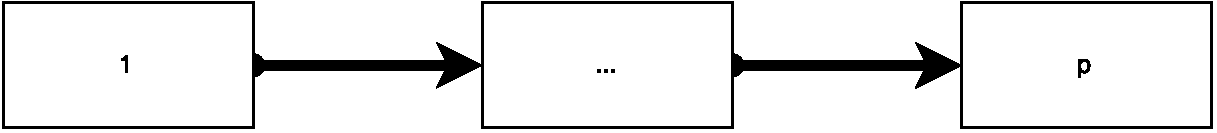
\includegraphics[width=0.7\linewidth]{art/series_system}
\caption{Series system.}
\label{fig:series_system}
\end{figure}


\begin{definition}[Parallel System]
A \emph{parallel system} is one where all components need to fail for the system to fail:
$$\struct(x)=1-\prod_{j=1}^{p} (1-x_j)= \coprod_{j=1}^p x_j.$$
\end{definition}
A reliability diagram of a parallel system is given in Figure~\ref{fig:parallel_system}.
\begin{figure}[ht]
\centering
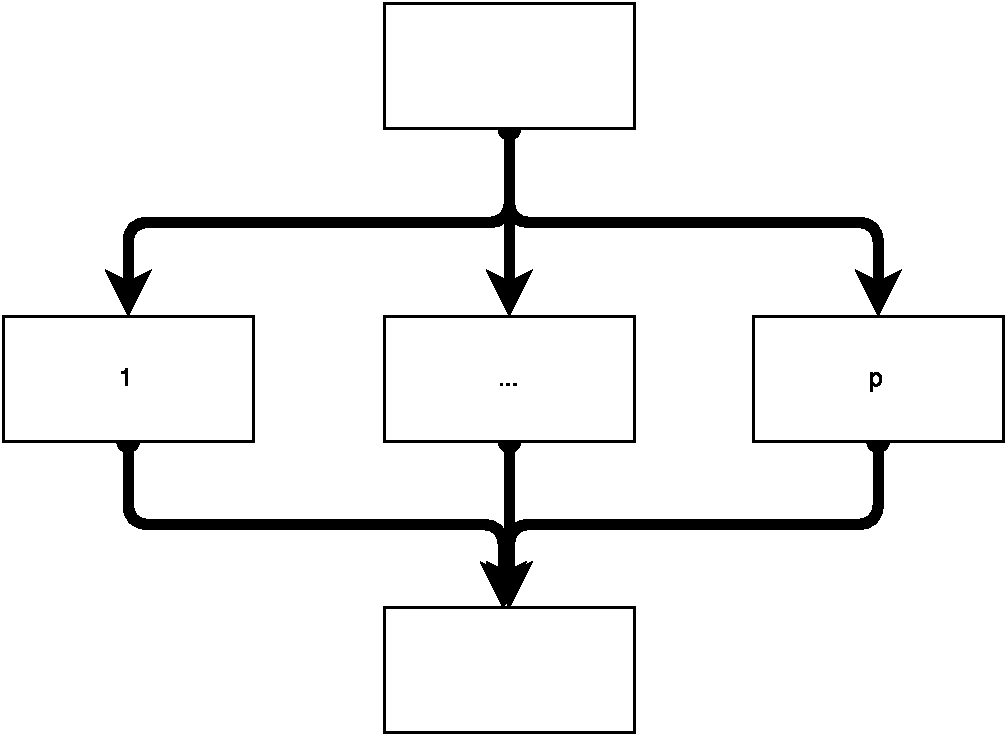
\includegraphics[width=0.7\linewidth]{art/parallel_system}
\caption{Parallel system.}
\label{fig:parallel_system}
\end{figure}


\begin{definition}[k-out-of-p System]
A \emph{k-out-of-p} system is one where at least $k+1$ components need to fail for the system to fail:
$$\struct(x)=\indicator{\sum_{j=1}^{p} x_j \geq k}.$$
\end{definition}
A reliability diagram of a k-our-of-p system is not provided, since it is not very friendly.




\begin{definition}[Monotone System]
A system is said to be \emph{monotone} if $\struct(x_1,\dots,\x_p)$ is non decreasing in all is components.
\end{definition}
The definition of monotonicity captures the idea that you cannot improve a system's state by breaking components.
This seems rather natural (I am still looking for a counter example).






\begin{definition}[Reliability]
We define the \emph{reliabity of component $j$} to be $$p_j:= P(\x_j=1),$$ 
and  the \emph{reliability of the system} 
$$ S_\struct:=P(\struct(x)=1).$$
\end{definition}


\begin{example}[Reliability of a series system]
For $\Phi(x)$ a series system, assuming independent components, we have
$$ S_\struct= \prod_{j=1}^{p} p_j.$$
\end{example}


\begin{example}[Reliability of a parallel system]
For $\Phi(x)$ a parallel system, assuming independent components, we have
$$ S_\struct= 1-\prod_{j=1}^{p} (1-p_j)= \coprod_{j=1}^p p_j. $$
\end{example}


\begin{example}[Reliability of a k-out-of-p system]
For $\Phi(x)$ a k-out-of-p system, assuming independent components with equal reliability ($p_i=p$), we have
$$ S_\struct= \sum_{i=k}^{p} \binom{n}{i} p^i (1-p)^{n-i} .$$
\end{example}


\begin{extra}[Reliability analysis of complex systems]
Except for simple systems, of the type we presented, the computation of the reliability of a complex system may be a formidable task. 
For complicated real-life systems, \emph{mix-cut--max-flow} algorithms, or \emph{inclusion-exclusion} type algorithms are emplyed. 
For more details, see \cite{aven_stochastic_1999}.
\end{extra}



\subsection{A Time Dynamic View}
The reliability of each component ($p_j$), typically changes in time, and so does the reliability of the whole system.
In the following, $\T$ will typically stand for the time to malfunction. It is thus assumed to be \textbf{continuous} and \textbf{non-negative}.


\begin{definition}[CDF]
The cumulative distribution function (CDF) of a random variable $\T$ at a point $t$  is given by
\begin{align}
	\cdf{\T}{t}:= P(\T<t).
\end{align}
\end{definition}

\begin{definition}[PDF]
The probability density function (PDF) of a continuous random variable $\T$ at a point $t$ is given by 
\begin{align}
	\pdf{\T}{t}:= \frac{\partial}{\partial t}\cdf{\T}{t}.
\end{align}
\end{definition}


\begin{definition}[Survival Function]
The survival function of a random variable $\T$ at a point $t$ is given by 
\begin{align}
	\survive{\T}{t}:= P(\T>t)=1-\cdf{\T}{t}.
\end{align}
\end{definition}
By definition, it follows that if $\T_j$ is the time to failure of component $j$, then $p_j(t)=\survive{\T_j}{t}$.
Our notation bot $S_\struct$ also becomes clear, since it $\T_\struct$ is the time to failure of a structure $\Phi$, then we may write $S_\struct(t)=\survive{\T_\struct}{t}$.


\begin{example}[Survival of a series system]
For a series system $\struct$, the reliability of the system at time $t$ is given by $$\survive{\Phi}{t}=\prod_{j=1}^{p} p_j(t)$$.
\end{example}


\begin{example}[Survival of a parallel system]
For a series system $\struct$, the reliability of the system at time $t$ is given by $$\survive{\Phi}{t}=\prod_{j=1}^{p} p_j(t)$$.
\end{example}





Another way to present a distribution, no less informative than the previous ones, is by the \emph{hazard function}, which is the ``probability of surviving just another instant''.
\begin{definition}[Failure Rate]
The \emph{hazard function}, or \emph{failure rate}, of a random variable $\T$ at a point $t$ is given by \marginnote{Hazard Function}
\begin{align}
	\hazard{\T}{t} &:= \lim_{dt\to 0}\frac{P( \T \in [t,t+dt)|\T \geq t )}{dt} \label{eq:hazard}\\
	&= \frac{\pdf{\T}{t}}{\survive{\T}{t}} \\
	&= \frac{\partial}{\partial t}\log \survive{\T}{t}.
\end{align}
\end{definition}





\begin{definition}[Cumulative Risk]
The \emph{cumulative hazard}, \aka the \emph{cumulative risk}, of a random variable $\T$ at a point $t$ is given by \marginnote{Cumulative Hazrd}
\begin{align}
	\cuhazard{\T}{t} &:= \int_{0}^{t}\hazard{\T}{t} \\
	\Rightarrow \survive{\T}{t} &= \exp(-\cuhazard{\T}{t}). \label{eq:cumhazrd}
\end{align}
\end{definition}
Eq.(\ref{eq:cumhazrd}) readily shows that a distribution is well defined by its hazards.



\begin{theorem}[Failure rate of a series system]
The failure rate of a series system of independent components $\Phi$ is given by the sum of the failure rates of its components
\begin{align}
	\hazard{\Phi}{t}= \sum_{j=1}^{p} \hazard{\T_j}{t}
\end{align}
\end{theorem}
The proof is immediate using the cumulative risk.
The failure rate of a parallel system, does not admit such a nice closed form.

\begin{example}[Exponential Hazard]
The simplest distribution when discussing hazards is the exponential.
Recalling
\begin{align}
	\pdf{\T}{t}= \lambda \exp(-\lambda t) \indicator{t \geq 0} \\
	\cdf{\T}{t}= (1-\exp(-\lambda t)) 
\end{align}
so that 
\begin{align}
	\survive{\T}{t} &= \exp(-\lambda t), \\
	\hazard{\T}{t} &= \lambda.
\end{align}
\end{example}
The exponential is the only distribution with constant hazard which makes it very easy to analyze.
The constant hazard is due to the \emph{memoryless} property; think what the memoryless property implies on Eq.(\ref{eq:hazard}).



\begin{example}[Failure rate of a series of exponential components]
The failure rate of a series system $\Phi$, of $p$ independent components each with exponentially distributed failure times, is simply 
\begin{align}
	\hazard{\Phi}{t}= p \lambda, \forall t \geq 0
\end{align}
\end{example}
This is obviously the simplest system possible for reliability analysis, which stems from the fact that a minimum of exponentials is exponential with the sum of rates.



The following example, seemingly very simple, provides tremendous insight into the complexities of reliability analysis.
\begin{example}[Failure rate of a two exponential-component parallel-system]
\label{eg:failure_parallel}
Consider a system of two independent, parallel, exponential components, with failure times $\T_j\sim \exp(\lambda_j); j=1,2$.
The failure rate is given by
\begin{align}
	\hazard{\Phi}{t}=
	\frac
	{\exppdf{\lambda_1}{t} + \exppdf{\lambda_2}{t}  - \exppdf{(\lambda_1+ \lambda_2)}{t}}
	{\expcdf{\lambda_1}{t} + \expcdf{\lambda_2}{t} - \expcdf{(\lambda_1+ \lambda_2)}{t}}
\end{align}
\end{example}
Why is Example~\ref{eg:failure_parallel} so important?
Because it a simple example that demonstrates a \textbf{non-monotone} failure rate, as depicted in Figure~\ref{fig:hazard_non_monotone}. 


\begin{figure}[ht]
\centering
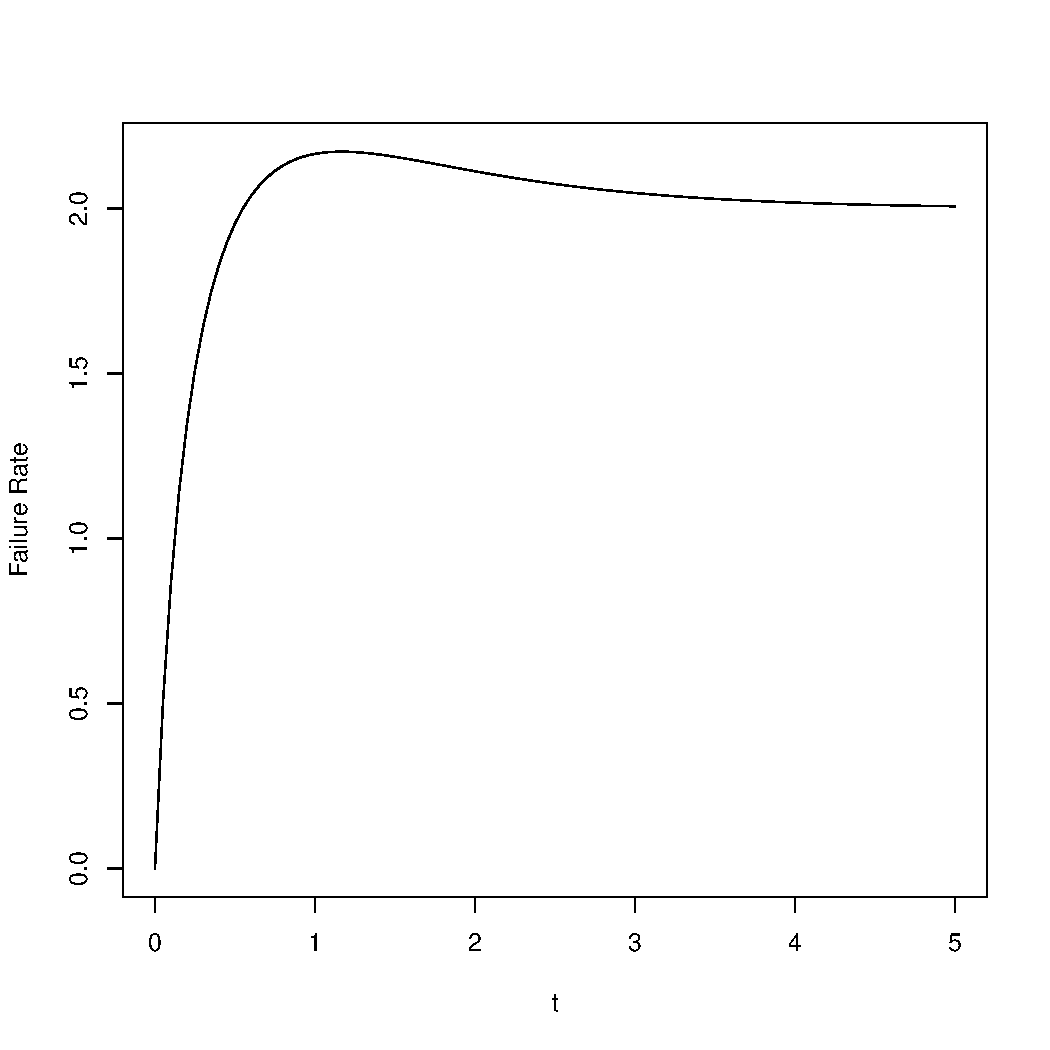
\includegraphics[width=0.7\linewidth]{art/hazard}
\caption{Failure rate of the parallel exponential component system.}
\label{fig:hazard_non_monotone}
\end{figure}





\begin{example}[Weibull Hazard]
The Weibull distribution is very common in reliability analysis, and can be constructed by 
$\T := \lambda \U^{1/k}$, where $\U \sim \exp(1)$. 
Recalling
\begin{align}
	\pdf{\T}{t} &= \frac{k}{\lambda}\left(\frac{\T}{\lambda} \right)^{k-1} \exp\left(-\frac{\T}{\lambda} \right)^k  \indicator{\T\geq 0} \\
	\cdf{\T}{t} &= 1 - \exp \left(-\frac{\T}{\lambda} \right)^k 
\end{align}
so that 
\begin{align}
	\survive{\T}{t} &= \exp \left(-\frac{\T}{\lambda} \right)^k \\
	\hazard{\T}{t} &= \frac{k}{\lambda} \left(\frac{\T}{\lambda} \right)^{k-1} .
\end{align}
\end{example}
Elementary analysis shows that the hazard function of the Weibull may be increasing or decreasing in time ($\T$), depending on $k$, but it is always monotone.




\begin{example}[Empirical risk rates]
When examining empirical risk rates of true devices, we almost always notice a \emph{bathtub} structure, such as in Figure~\ref{fig:bathtub}.
This shape captures the idea that products tend to fail more when they are brand new, or as they are very old, while their failure rates are fairly stable in the ``mid-life''.
In this text, we will not be providing a particular distribution which has this property. 
We refer the reader to \cite{nadarajah_bathtub-shaped_2008} for examples of distributions which have the bathtub property.
\end{example}


\begin{figure}[ht]
\centering
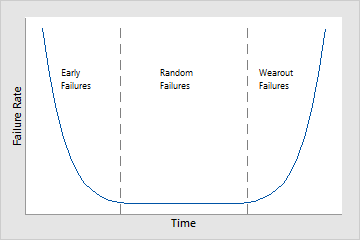
\includegraphics[width=0.7\linewidth]{art/bathtub_curve}
\caption{Bathtub curve of empirical failure rates. \newline
\url{http://support.minitab.com/en-us/minitab/17/topic-library/modeling-statistics/reliability/distributions-in-reliability-analysis/hazard-functions/}}
\label{fig:bathtub}
\end{figure}





\section{Statistical Analysis}
[TODO]


\section{Bibliographic Notes}
This chapter is adapted from \cite[Ch.8]{natrella_nist/sematech_2010}, German Rodriguez's Generalized-Linear-Models class notes\footnote{\url{http://data.princeton.edu/wws509/notes/c7.pdf}.}.
See \cite{aven_stochastic_1999} for a mathematically rigorous treatment.

